%% LyX 1.3 created this file.  For more info, see http://www.lyx.org/.
%% Do not edit unless you really know what you are doing.
\documentclass[english, 12pt]{article}
\usepackage{times}
%\usepackage{algorithm2e}
\usepackage{url}
\usepackage{bbm}
\usepackage[T1]{fontenc}
\usepackage[latin1]{inputenc}
\usepackage{geometry}
\geometry{verbose,letterpaper,tmargin=2cm,bmargin=2cm,lmargin=1.5cm,rmargin=1.5cm}
\usepackage{rotating}
\usepackage{color}
\usepackage{graphicx}
\usepackage{subcaption}
\usepackage{amsmath, amsthm, amssymb}
\usepackage{setspace}
\usepackage{lineno}
\usepackage{hyperref}
\usepackage{bbm}
\usepackage{makecell}

%\renewcommand{\arraystretch}{1.8}

\usepackage{xr}
\externaldocument{paper-ldpred2-supp}

%\linenumbers
%\doublespacing
\onehalfspacing
%\usepackage[authoryear]{natbib}
\usepackage{natbib} \bibpunct{(}{)}{;}{author-year}{}{,}

%Pour les rajouts
\usepackage{color}
\definecolor{trustcolor}{rgb}{0,0,1}

\usepackage{dsfont}
\usepackage[warn]{textcomp}
\usepackage{adjustbox}
\usepackage{multirow}
\usepackage{graphicx}
\graphicspath{{../figures/}}
\DeclareMathOperator*{\argmin}{\arg\!\min}
\usepackage{algorithm} 
\usepackage{algpseudocode} 

\let\tabbeg\tabular
\let\tabend\endtabular
\renewenvironment{tabular}{\begin{adjustbox}{max width=0.9\textwidth}\tabbeg}{\tabend\end{adjustbox}}

\makeatletter

%%%%%%%%%%%%%%%%%%%%%%%%%%%%%% LyX specific LaTeX commands.
%% Bold symbol macro for standard LaTeX users
%\newcommand{\boldsymbol}[1]{\mbox{\boldmath $#1$}}

%% Because html converters don't know tabularnewline
\providecommand{\tabularnewline}{\\}

\usepackage{babel}
\makeatother


\begin{document}


\title{LDpred2: better, faster, stronger}
\author{Florian Priv\'e,$^{\text{1,}*}$ Julyan Arbel,$^{\text{2}}$ and Bjarni J. Vilhj\'almsson$^{\text{1,3,}*}$}

\date{~ }
\maketitle

\noindent$^{\text{\sf 1}}$National Centre for Register-Based Research, Aarhus University, Aarhus, 8210, Denmark. \\
\noindent$^{\text{\sf 2}}$Univ.\ Grenoble Alpes, Inria, CNRS, Grenoble INP, LJK, Grenoble, 38000, France. \\
\noindent$^{\text{\sf 3}}$Bioinformatics Research Centre, Aarhus University, Aarhus, 8000, Denmark. \\
\noindent$^\ast$To whom correspondence should be addressed.\\

\noindent Contacts:
\begin{itemize}
\item \url{florian.prive.21@gmail.com}
\item \url{bjv@econ.au.dk}
\end{itemize}

\vspace*{4em}

\abstract{	

}


%%%%%%%%%%%%%%%%%%%%%%%%%%%%%%%%%%%%%%%%%%%%%%%%%%%%%%%%%%%%%%%%%%%%%%%%%%%%%%%%

\clearpage

\section{Introduction}

In recent years the use of polygenic scores (PGS) has become widespread. A PGS aggregates (risk) effects across many genetic variants into a single predictive score. These scores have proven useful for studying the genetic architecture and relationships between diseases and traits \cite[]{purcell2009common,kong2018nature}.
Moreover, there are high hopes for using these scores in clinical practice to improve disease risk estimates and prognostic accuracies.
The heritability, i.e.\ the proportion of phenotypic variance that is attributable to genetics, determines an upper limit on the predictive performance of PGS and thus their value as a diagnostic tool.
Nevertheless, a number of studies have explored the use of PGS in clinical settings \cite[]{pashayan2015implications,willoughby2019genetic,abraham2019genomic}.
PGS are also extensively used in epidemiology and economics as predictive variables of interest [TODO BJARNI CITATIONS]. 
For example, a recently derived PGS for education attainment has been one of the most predictive variables in behavioural sciences so far \cite[]{allegrini2019genomic}.

LDpred is a popular and powerful method for deriving polygenic scores based on summary statistics and a Linkage Disequilibrium (LD) matrix only \cite[]{vilhjalmsson2015modeling}.
It assumes there is a proportion $p$ of variants that are causal.
However, LDpred has several limitations that may result in limited predictive performance.
The non-infinitesimal version of LDpred, a Gibbs sampler, is particularly sensitive to model misspecification when applied to summary statistics with large sample sizes.
It is also unstable in long-range LD regions such as the human leukocyte antigen (HLA) region of chromosome 6. 
This issue has lead to the removal of such regions from analyses  \cite[]{marquez2018modeling,lloyd2019improved}, which is unfortunate since this region of the genome contains many known disease-associated variants, particularly with autoimmune diseases and psychiatric disorders \cite[]{mokhtari2016major,matzaraki2017mhc}.
%LDpred is also considered not particularly fast, nor memory-efficient, nor it provides truly sparse models as expected by its model specification.

Here, we present LDpred2, a new version of LDpred that addresses these issues while markedly improving its computational efficiency.
We provide this faster and more robust implementation of LDpred in R package bigsnpr \cite[]{prive2017efficient}.
We also provide two new options in LDpred2. First, we provide a ``sparse'' option, where LDpred2 truly fits some effects to zero, therefore providing a sparse vector of effects. Second, we also provide an ``auto'' option, where LDpred2 automatically estimates the sparsity $p$ and the SNP heritability $h^2$, and therefore does not require validation data to tune hyper-parameters.
We show that LDpred2 provides higher predictive performance than LDpred1 (LDpred v1.0.0), especially when there are causal variants in long-range LD regions, or when the proportion of causal variants is small.
We also show that the new sparse option performs equally well as the non-sparse version, enabling LDpred2 to provide sparse effects without losing prediction accuracy.


%%%%%%%%%%%%%%%%%%%%%%%%%%%%%%%%%%%%%%%%%%%%%%%%%%%%%%%%%%%%%%%%%%%%%%%%%%%%%%%%

\section{Results}

\subsection*{Overview of methods}

Here we present LDpred2, a new version of LDpred \cite[]{vilhjalmsson2015modeling}.
LDpred2 has 4 options: 1) LDpred2-inf, an infinitesimal model similar to the one in LDpred1; 2) LDpred2-grid (or simply LDpred2) that is the main LDpred model, where a grid of values for hyper-parameters $p$ (the proportion of causal variants) and $h^2$ (the SNP heritability) are tuned using a validation test; 3) LDpred2-sparse, which is similar to LDpred2-grid but where effects can be exactly 0, offering a truly sparse version of LDpred; 4) LDpred2-auto, which automatically estimate $p$ and $h^2$ and therefore is free of hyper-parameters to optimize.
As a recall, LDpred v1 has two options: LDpred1-grid where only $p$ is optimized, and LDpred1-inf.

We compare the two versions of LDpred using six simulation scenarios to understand in which cases it is important to use the new version. We also compare these two versions of LDpred using eight binary phenotypes of major interest and for which there are published external summary statistics available and a substantial number of cases in the UK Biobank data. Area Under the ROC Curve (AUC) values are reported.

\subsection*{Simulations}

Figure \ref{fig:AUC-simu} presents the simulation results comparing LDpred1 (v1.0.0 as implemented by \cite{vilhjalmsson2015modeling}) with the new LDpred2 (as implemented in R package bigsnpr). 
six simulation scenarios are used, each repeated 10 times.
In the first four simulation scenarios, a heritability $h^2$ of 40\% and a prevalence of 15\% are used. We simulate 300, 3000, 30,000 or 300,000 causal variants anywhere on the genome. 
In these scenarios, infinitesimal models perform similarly. 
When testing a grid of hyper-parameters, LDpred2 performs substantially better than LDpred1 in the cases where the number of causal variants is smaller, i.e.\ in the case of 300 or 3000 causal variants ($p$=2.5e-4 and 2.5e-3). 
For example, in simulations with 300 causal variants, a mean AUC of 73.5\% is obtained with LDpred1 while a value of 81.9\% is obtained with LDpred2.
In these scenarios, all 3 non-infinitesimal models of LDpred2 perform equally well.
In HLA scenarios, i.e.\ when causal variants are sampled in a region with variants in high LD, LDpred1 performs poorly. In these two HLA scenarios, all LDpred2 models perform well, although LDpred2-auto performs slightly worse than other models.

%% FIGURE 1 HERE
\begin{figure}[h]
\centerline{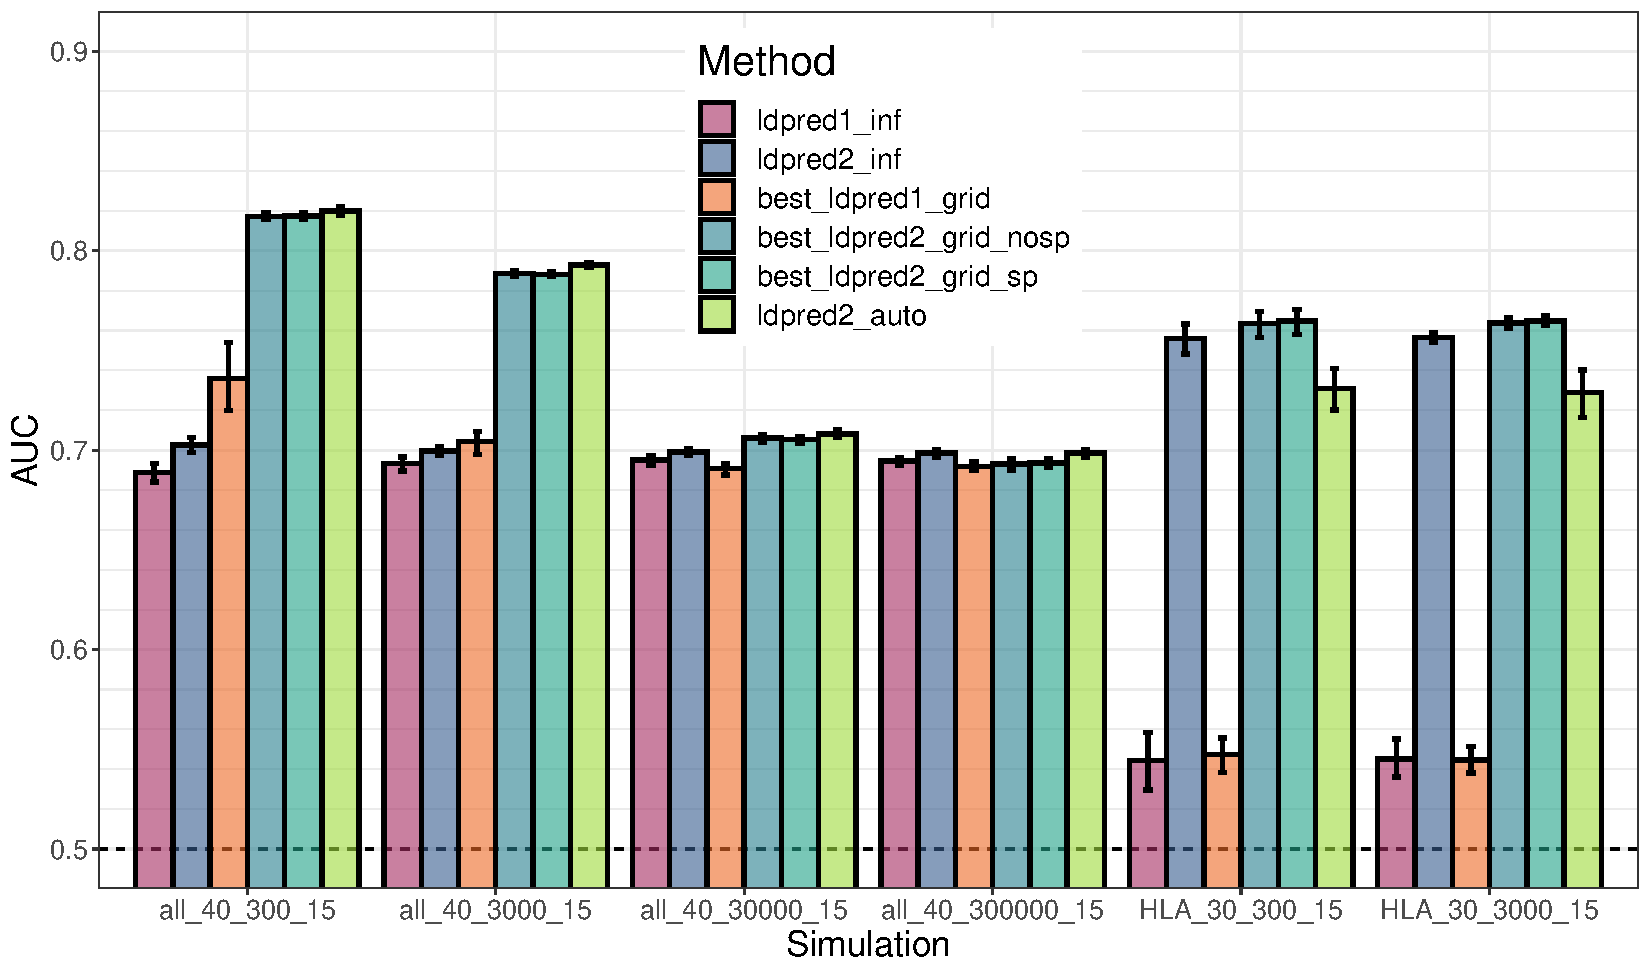
\includegraphics[width=0.95\textwidth]{AUC-simu}}
\caption{Results of the six simulation scenarios. 
Scenarios are named in 4 parts separated by underscores: 1) ``all'' means that causal variants are randomly sampled anywhere on the genome while ``HLA'' means that they are sampled in the HLA region of chromosome 6 (25-35 Mb); 2) the heritability (in \%); 3) the number of causal variants; 4) the prevalence (in \%).
Bars present the mean and 95\% CI of $10^4$ non-parametric bootstrap replicates of the mean AUC of 10 simulations for each scenario. 
%See corresponding values in table S1.
}
\label{fig:AUC-simu}
\end{figure}

\subsection*{Real data}

Figure \ref{fig:AUC-real} presents the results of real data applications comparing LDpred1 (v1.0.0 as implemented by \cite{vilhjalmsson2015modeling}) with the new LDpred2 (as implemented in R package bigsnpr). 
eight binary phenotypes are used, summarized in table \ref{tab:sumstats}.
For T1D, T2D, BRCA, PRCA and MDD, all LDpred2 models perform much better than LDpred1. For example, for BRCA, AUC improves from 58.5\% with LDpred1 to 65\% with LDpred2, and from 55\% to 75\% for T1D. 
For Asthma, CAD and RA, predictive performances of LDpred1 and LDpred2 are similar.

As in simulations, the sparse version of LDpred2 performs equally well as the original version, with the exception of PRCA, for which it performs poorly.
For CAD, PRCA and TD1, LDpred2-auto perform much worse than LDpred2, otherwise it performs similarly.

%% FIGURE 2 HERE
\begin{figure}[h]
\centerline{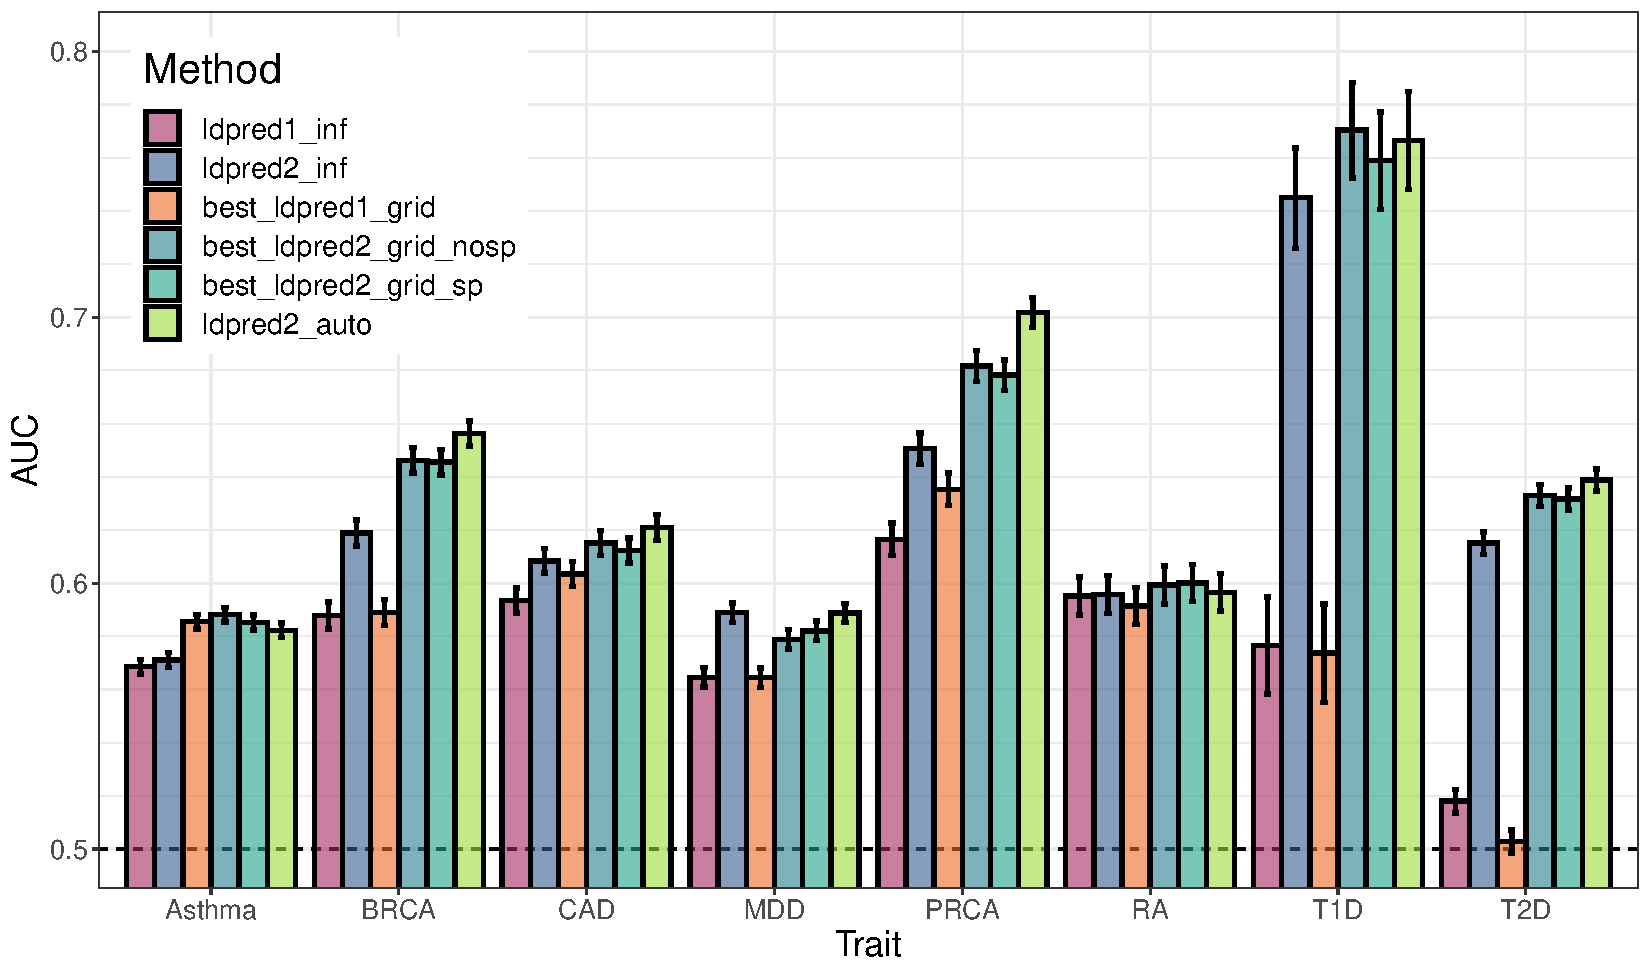
\includegraphics[width=0.85\textwidth]{AUC-real}}
\caption{Results of the real data applications using published external summary statistics.
Bars present AUC values on the test set of UKBB (mean and 95\% CI from $10^4$ bootstrap samples).
%See corresponding values in table S2.
}
\label{fig:AUC-real}
\end{figure}

%%%%%%%%%%%%%%%%%%%%%%%%%%%%%%%%%%%%%%%%%%%%%%%%%%%%%%%%%%%%%%%%%%%%%%%%%%%%%%%%

\section{Discussion}

Here we present LDpred2, a new version of LDpred. 
LDpred is widely used and has the potential to provide polygenic models with good predictive performance \cite[]{khera2018genome}. 
Yet, it has some instability issues that have been pointed out \cite[]{marquez2018modeling,lloyd2019improved} and likely contributed to discrepancies in reported prediction accuracies \cite[]{choi2019prsice,ge2019polygenic}.
We propose a new version of LDpred to solve these instability issues and improve its computational efficiency.

We show that LDpred2 is much more stable and provides higher prediction than LDpred1.
We demonstrate that LDpred1 has defects, particularly when handling long-range LD regions such as the HLA region.
Indeed, LDpred1 performs poorly in the simulations where causal variants are in the HLA region.
In contrast, LDpred2 performs very well. We hypothesize that LDpred1 does not use a window size that is large enough to account for long-range LD such as in the HLA region.
In LDpred2, we use a window size of 3 cM, which is much larger than the default value used in LDpred1 and which enables LDpred2 to work well even when causal variants are in long-range LD regions.
%We hypothesize that using a larger LD window explains the 5 real traits where LDpred2 performs much better than LDpred1, especially because LDpred2-inf performs better than LDpred1-inf.
We strongly discourage against removing these regions as sometimes suggested in the literature. 
Indeed, these regions, especially the HLA region, contain lots of variants associated with many traits, and are therefore very useful for prediction.

In LDpred2, we also test more values for $p$ (17 instead of 7 by default) and for $h^2$ (3 instead of 1).
When testing the grid of hyper-parameters of $p$ and $h^2$, we also allow for testing an option to enable sparse models in LDpred2 (see after).
Overall, we test a grid of 102 different values in LDpred2 instead of 7 in LDpred1, we use 5 times as many iterations in the Gibbs sampler, we use a larger window size for computing correlation, yet LDpred2 is still as fast as LDpred1.
LDpred2 is fast because we provide an efficient parallel implementation in C++. The parallelization is performed on the grid of hyper-parameters, but can also be performed chromosome-wise, as each chromosome is processed independently in LDpred2 (see Methods).
As an example, it takes less than two hours to run LDpred2-inf, LDpred2-grid (108 hyper-parameter values) and LDpred2-auto for a chromosome with 100K variants and using 8 cores.
Pre-computing the LD matrix for a chromosome with 100K variants takes 11 minutes using 16 cores.

LDpred2 also comes with two new models.
When the sparse option is enabled, it provides models that truly encourage sparsity, as compared to LDpred1 which outputs very small non-zero effect sizes \cite[]{cecile2019polygenic}.
It can provide sparsity in effect sizes as much as 98\% for small $p$, while keeping predictive performance as good as non-sparse models, as opposed to if very small effects were simply discarded \cite[]{bolli2019software}.
This sparse model performs equally well as the non-sparse model, therefore we encourage users to test it in the grid and to choose it if it performs equally well as the non-sparse model.
As for LDpred2-auto, which automatically estimates values for hyper-parameters $p$ and $h^2$, it performs equally well as other LDpred2 models in simulations, but does not perform well for half of the real traits analyzed here.
More investigations need to be performed to understand the poor results of LDpred2-auto for these particular real traits.

\begin{figure}[h]
	\centerline{\includegraphics[width=0.85\textwidth]{QC-CAD}}
	\caption{Results of the real data applications using published external summary statistics.
		Bars present AUC values on the test set of UKBB (mean and 95\% CI from $10^4$ bootstrap samples).
		%See corresponding values in table S2.
	}
	\label{fig:QC-CAD}
\end{figure}
[TALK ABOUT QUALITY CONTROL ON AF?]

[TALK ABOUT DIFFERENT SETS OF VARIANTS?]


%%%%%%%%%%%%%%%%%%%%%%%%%%%%%%%%%%%%%%%%%%%%%%%%%%%%%%%%%%%%%%%%%%%%%%%%%%%%%%%%

\section{Methods}

\subsection*{Simulation analyses}

We use the UK Biobank data for both real data analyses and simulations \cite[]{bycroft2018uk}. We restrict individuals to White-British individuals used in the PC computation of the UK Biobank (i.e.\ unrelated and quality-controlled). We restrict variants to HapMap3 variants (considered to be well imputed).
This results in 337,475 individuals and 1,194,574 variants.
We use 10,000 individuals as a validation set for choosing optimal hyper-parameters and for computing correlations between variants (LD matrix). 
We use 300,000 other individuals for running logistic GWAS to create summary statistics.
We use the remaining 27,475 individuals as test set for evaluating models.

We simulate binary phenotypes with a heritability of $h^2 = 0.4$ (or 0.3)  using a Liability Threshold Model (LTM) with a prevalence of 15\% \cite[]{falconer1965inheritance}. 
We vary the number of causal variants (300, 3000, 30,000, or 300,000) to match a range of genetic architectures from low to high polygenicity.
Liability scores are computed from a model with additive effects only: we compute the liability score of the $i$-th individual as \(y_i = \sum_{j\in S_\text{causal}} w_j \widetilde{G_{i,j}} + \epsilon_i,\) where $S_\text{causal}$ is the set of causal variants, $w_j$ are weights generated from a Gaussian distribution $N(0, h^2 / \vert S_\text{causal} \vert)$, $G_{i,j}$ is the allele count of individual $i$ for variant $j$, $\widetilde{G_{i,j}}$ corresponds to its standardized version (zero mean and unit variance), and $\epsilon_i$ follows a Gaussian distribution $N(0, 1 - h^2)$.
Causal variants are chosen randomly anywhere on the genome. 
We make two other simulation scenarios with 300 or 3000 causal variants randomly chosen in the HLA region (chromosome 6, 25-35 Mb).
Both parts of the $y_i$'s are scaled such that the variance of the genetic liability is exactly $h^2$ and the variance of the total liability is exactly $1$. 
Such simulation of phenotypes based on real genotypes is implemented in function \texttt{snp\_simuPheno} of R package bigsnpr.
Each simulation scenario is repeated 10 times and averages of the Area Under the ROC Curve (AUC) are reported. 


\subsection*{Real data analyses}

We use the same data as in the simulation analyses. We use the same 10,000 individuals as validation set, and use the remaining 327,475 individuals as test set.
We use external published GWAS summary statistics listed in table \ref{tab:sumstats}.
We defined phenotypes as in \cite{prive2019making}. For details, please refer to our R code (Software and code availability section).

%% TABLE 1 HERE
\begin{table}[h]
	\centering
	\begin{tabular}{|l|c|c|c|c|}
		\hline
		Trait & GWAS citation & GWAS sample size & GWAS \#variants \\
		\hline
		Breast cancer (BRCA) & \cite{michailidou2017association} & 137,045 / 119,078 & 11,792,542 \\
		Rheumatoid arthritis (RA) & \cite{okada2014genetics} & ~~29,880 / ~~73,758 & ~~9,739,303 \\
		Type 1 diabetes (T1D) & \cite{censin2017childhood} & ~~~~~5913 / ~~~~~8828  & ~~8,996,866 \\
		Type 2 diabetes (T2D) & \cite{scott2017expanded} & ~~26,676 / 132,532 & 12,056,346 \\
		Prostate cancer (PRCA) & \cite{schumacher2018association} & ~~79,148 / ~~61,106 & 20,370,946 \\
		Depression (MDD) & \cite{wray2018genome} & ~~59,851 / 113,154 & 13,554,550 \\
		Coronary artery disease (CAD) & \cite{nikpay2015comprehensive} & ~~60,801 / 123,504 & ~~9,455,778 \\
		Asthma & \cite{demenais2018multiancestry} & ~~19,954 / 107,715 & ~~2,001,280 \\
		\hline
	\end{tabular}
	\caption{Summary of external GWAS summary statistics used. The GWAS sample size is the number of cases / controls in the GWAS. \label{tab:sumstats}}
\end{table}


\subsection*{From marginal effects to joint effects}

In this section, we explain how we can obtain joint effects from summary statistics (marginal effects) and a correlation matrix.
Let us denote by $S$ the diagonal matrix with standard deviations of the $m$ variants, $C_n = I_n - 1 1^T / n$ the centering matrix, $G$ the genotype matrix of $n$ individuals and $m$ variants, and $y$ the phenotype vector for $n$ individuals.

When solving a joint model with all variants and an intercept ${\alpha}$, the joint effects ${\gamma}_{\text{joint}}$ are obtained by solving
\[\begin{bmatrix} \hat{\alpha} \\ \hat{\gamma}_{\text{joint}} \end{bmatrix} = \left(\begin{bmatrix} 1 & G \end{bmatrix}^T \begin{bmatrix} 1 & G \end{bmatrix}\right)^{-1} \begin{bmatrix} 1 & G \end{bmatrix}^T y ~.\]
Using the Woodburry formula, we get 
\[\hat{\gamma}_{\text{joint}} = (G^T C_n G)^{-1} G^T C_n y ~.\]
When fitting each variant separately in GWAS, the marginal effects (assuming no covariate) simplify to 
\[\hat{\gamma}_{\text{marg}} = \dfrac{1}{n-1} S^{-2} G^T C_n y ~.\] 
We further note that the correlation matrix of $G$ is \(K =  \dfrac{1}{n-1} S^{-1} G^T C_n G  S^{-1}\).
Then we get \[\hat{\gamma}_{\text{joint}} = S^{-1} K^{-1} S \hat{\gamma}_{\text{marg}} ~.\]

For one marginal effect $\hat{\gamma}$, let us denote by $y^*$ and $g^*$ the corresponding phenotype and genotype (residualized from $K$ covariates, e.g.\ centering them).
Then,
$\text{var}(\hat{\gamma}) = \dfrac{(y^* - \hat{\gamma} g^*)^T (y^* - \hat{\gamma} g^*)}{(N - K - 1) ~ g^{*T} g^*} \approx \dfrac{y^{*T} y^*}{N ~ g^{*T} g^*} \approx \dfrac{\text{var}(y)}{N ~ \text{var}(g)}$.
Thus, we can derive $\text{sd}(g) \approx \dfrac{\text{sd}(y)}{\text{sd}(\hat{\gamma}) ~ \sqrt{N}}$ and $\left(\text{sd}(g) ~ \hat{\gamma}\right) \approx \dfrac{\hat{\gamma}}{\text{sd}(\hat{\gamma})} \dfrac{\text{sd}(y)}{\sqrt{N}}$.

Let us go back to the formula we derived before: $\hat{\gamma}_{\text{joint}} = S^{-1} K^{-1} S \hat{\gamma}_{\text{marg}}$. 
Note that $\gamma$ are the effects on the allele scale while we denote by $\beta = S \gamma$ the effects of the scaled genotypes.
As $\text{sd}(y)$ is the same for all variants, it is cancelled out by $S^{-1}$ and $S$. Then it justifies the use of Z-scores ($\hat{\gamma} ~/~ \text{sd}(\hat{\gamma})$) divided by $\sqrt{N}$ as input for LDpred. Then, the effect sizes that LDpred outputs need to be scaled by multiplying by $\left(\text{sd}(\hat{\gamma}) ~ \sqrt{N}\right)$.
Note that LDpred1 and other similar methods scale the output dividing by the standard deviation of genotypes. This is correct when $\text{sd}(y) = 1$ only.



\subsection*{Overview of LDpred model}

LDpred assumes the following model for effect sizes,
\begin{equation}\label{eq:model}
\beta_j = S \gamma_j \sim \left\{
\begin{array}{ll}
\mathcal N\left(0, \dfrac{h^2}{M p}\right) & \mbox{with probability $p$,} \\
0 & \mbox{otherwise,}
\end{array}
\right.
\end{equation}
where $p$ is the proportion of causal variants, $M$ the number of variants and $h^2$ the (SNP) heritability.
\cite{vilhjalmsson2015modeling} estimates $h^2$ using constrained LD score regression (intercept fixed to 1) and recommend testing a grid of hyper-parameter values for $p$ (1, 0.3, 0.1, 0.03, 0.01, 0.003 and 0.001).

\newcommand{\hmpn}{\dfrac{h^2}{M p} + \dfrac{1}{N}}
\newcommand{\phmpn}{\dfrac{p}{\sqrt{\hmpn}}}
\newcommand{\betahmpn}{\dfrac{\tilde{\beta}_j^2}{\hmpn}}

To estimate effect sizes $\beta_j$, \cite{vilhjalmsson2015modeling} use a Gibbs sampler, as described in algorithm \ref{algo:ldpred}.

First, they estimate the residualized marginal effect for variant $j$ as [SHOULD VERIFY]
\begin{equation}\label{eq:beta_res}
\tilde{\beta}_j = \hat{\beta}_j - \boldsymbol{\beta}^T_{\text{-}j} \boldsymbol{K}_{\text{-}j, j}
\end{equation}
where $\boldsymbol{K}_{\text{-}j, j}$ is the $j$-th column without the  $j$-th row of the correlation matrix and $\boldsymbol{\hat{\beta}}$ are the marginal effect sizes.
Then, they compute the probability that variant $j$ is causal as 
\[\bar{p}_j = P\left(\beta_j \sim \mathcal N(\cdot,\cdot) ~|~ \tilde{\beta}_j\right) = \dfrac{\phmpn \exp\left\lbrace-\dfrac{1}{2} \betahmpn\right\rbrace}{\phmpn \exp\left\lbrace-\dfrac{1}{2} \betahmpn\right\rbrace + \dfrac{1-p}{\sqrt{\dfrac{1}{N}}} \exp\left\lbrace-\dfrac{1}{2} \dfrac{\tilde{\beta}_j^2}{\dfrac{1}{N}}\right\rbrace}~,\]
which we rewrite as
\begin{equation}
\bar{p}_j = \dfrac{1}{1 + \dfrac{1-p}{p} \sqrt{1 + \dfrac{N h^2}{Mp}} \exp\left\lbrace-\dfrac{1}{2} \dfrac{N \tilde{\beta}_j^2}{1 + \dfrac{Mp}{N h^2}}\right\rbrace}~.\label{eq:postp}
\end{equation}
Computing $\bar{p}_j$ using the second expression is important to avoid numerical issues when $N \tilde{\beta}_j^2$ is large.

Then, $\beta_j$ is sampled according to
\begin{equation}\label{eg:random_beta}
\beta_j ~|~ \tilde{\beta}_j \sim \left\{
\begin{array}{ll}
\mathcal N\left(\dfrac{1}{1 + \dfrac{M p}{N h^2}} \tilde{\beta}_j, \dfrac{1}{1 + \dfrac{M p}{N h^2}}\dfrac{1}{N}\right) & \mbox{with probability $\bar{p}_j$,} \\
0 & \mbox{otherwise.}
\end{array}
\right.
\end{equation}

Therefore, the posterior mean of $\beta_j$ is given by 
\begin{equation}\label{eg:post_beta}
\omega_j = \dfrac{\bar{p}_j \tilde{\beta}_j}{1 + \dfrac{M p}{N h^2}} ~.
\end{equation}

%\begin{minipage}{.7\textwidth}
\begin{algorithm}[H]
\caption{LDpred, with hyper-parameters $p$ and $h^2$}\label{algo:ldpred}
\begin{algorithmic}[1]
	\State $\boldsymbol{\hat{\beta}} \gets \dfrac{\boldsymbol{\hat{\gamma}}}{\boldsymbol{\text{sd}(\hat{\gamma})} \cdot \sqrt{\boldsymbol{N}}}$ \Comment{See previous section}
	\State $\boldsymbol{\Omega} \gets \boldsymbol{0}$
	\For {$k=1,\ldots,N_\text{burn-in} + N_\text{iter}$} \Comment{Gibbs iterations}
	\For {each variant $j$} \Comment{All variants}
	\State Compute $\tilde{\beta}_j$ according to \eqref{eq:beta_res}
	\State Compute $\bar{p}_j$ according to \eqref{eq:postp}
	\State Sample $\beta_j$ according to \eqref{eg:random_beta}
	\State Compute $\omega_j$ according to \eqref{eg:post_beta}
	\EndFor
	\State Compute $\boldsymbol{\beta}^T \boldsymbol{K} \boldsymbol{\beta}$ (estimate of $h^2$) to check divergence \Comment{Return 0s if divergence}
	\If {$k > N_\text{burn-in}$} 
	\State Increment $\boldsymbol{\Omega}$ with $\boldsymbol{\omega}$ 
	\EndIf
	\EndFor
	\State $\boldsymbol{\Omega} \gets \boldsymbol{\Omega} /  N_\text{iter}$
	\State Return $\boldsymbol{\Omega} \cdot  \boldsymbol{\text{sd}(\hat{\gamma})} \cdot \sqrt{\boldsymbol{N}}$ \Comment{See previous section}
\end{algorithmic} 
\end{algorithm}
%\end{minipage}

[CHANGE NOTATION OF SUMSTATS / SD -> SE?]

\subsection*{New LDpred2 models}

LDpred2 comes with two extensions of the LDpred model.

The first extension consists in estimating $p$ and $h^2$ in the model, as opposed to testing several values of $p$ and estimating $h^2$ using constrained LD score regression \cite[]{bulik2015ld}. This makes LDpred2-auto a method free of hyper-parameters which can therefore directly be applied to data without the need of a validation dataset to choose best-performing hyper-parameters.
To estimate $p$, we count the number of causal variants (i.e.\ $m_c = \sum_j(\beta_j \neq 0)$ in equation \ref{eg:random_beta}). 
We can assume that $m_c \sim \text{Binom}(M, p)$, so if we place a prior $p \sim \text{Beta}(1, 1) \equiv \mathcal{U}(0, 1)$, we can sample $p$ from the posterior $p \sim \text{Beta}(1 + m_c, 1 + M - m_c)$.
Due to complexity reasons, we could not derive a Bayesian estimator of $h^2$. Instead, we estimate $h^2 = \beta^T K \beta$, where $K$ is the correlation matrix.
These parameters $p$ and $h^2$ are updated after the inner loop in algorithm \ref{algo:ldpred}, then these new values are used in the next iteration of the outer loop.

The second extension, LDpred2-sparse, aims at providing sparse effect size estimates, i.e.\ that some resulting effects are exactly 0.
When the sparse solution is sought and when $\bar{p}_j < p$, we set $\beta_j$ and $\omega_j$ to 0 (lines 6-8 of algorithm \ref{algo:ldpred}).
Note that LDpred2-auto does not have a sparse option, but it is possible to run LDpred2-sparse with the $p$ and $h^2$ estimates from LDpred2-auto.

\subsection*{New strategy for local correlation}

LDpred has a window size parameter that needs to be set; for a given variant, correlations with other variants outside of this window are assumed to be 0.
The recommended value for this window (in number of variants) is to use the total number of variants divided by 3000, which corresponds to a window radius of around 2 Mb \cite[]{vilhjalmsson2015modeling}.
We have come to the conclusion that this window size is not large enough. Indeed, the human leukocyte antigen (HLA) region of chromosome 6 is 8 Mb long \cite[]{price2008long}. 
Using a window of 8Mb would be computationally and memory inefficient.
Instead, we propose to use genetic distances. Genome-wide, 1 Mb corresponds on average to 1 cM. Yet, the HLA region is only 3 cM long (vs.\ 8 Mb long).
Therefore, genetic distances enable to capture the same LD using a globally smaller window.
We provide function \texttt{snp\_asGeneticPos} in package bignspr to easily interpolate physical position to genetic positions.
We recommend to use genetic positions and to use a size parameter of 3 cM when computing the correlation between variants for LDpred2. 
Note that, in the code, we use \texttt{size = 3 / 1000} since parameter \texttt{size} is internally multiplied by 1000 in functions of package bigsnpr.
To prevent storing very small correlations, we also set to 0 all correlations with a p-value larger than \texttt{alpha = 0.9} (when testing that the correlation is different from 0).

\subsection*{New strategy for running LDpred2}

We recommend to run LDpred2 per chromosome.
Even if it is possible to run LDpred2 genome-wide, this approach has two limitations. First, it can be memory and computationally demanding to do so. For around one million (1M) variants, storing the 1M$\times$1M sparse correlation matrix takes more than 32 GB of memory. 
Doubling to 2M variants would require 128 GB of RAM to store the matrix.
Second, as noted in \cite{prive2019making}, it may be beneficial to assume that architecture of traits may be different for different chromosomes.
For example, autoimmune diseases clearly show larger effects on chromosome 6 compared to other chromosomes.
Assuming the same model for genetic effects genome-wide could result in severe model misspecification, which would lead to suboptimal predictive performance.
Moreover, since the inverse of a block-diagonal matrix is formed from the inverse of each block, it should be safe to run LDpred2 for each chromosome and then combine the results.  


%%%%%%%%%%%%%%%%%%%%%%%%%%%%%%%%%%%%%%%%%%%%%%%%%%%%%%%%%%%%%%%%%%%%%%%%%%%%%%%%

\clearpage
%\vspace*{5em}

\section*{Software and code availability}

[TODO] 
All code used for this paper is available at \url{https://github.com/privefl/paper-ldpred2/tree/master/code}.
R package bigsnpr can be installed from either CRAN or GitHub (see \url{https://github.com/privefl/bigsnpr}).
A tutorial on the steps to run LDpred2 using some small example data is available at \url{https://privefl.github.io/bigsnpr/articles/LDpred2.html}. 

\section*{Acknowledgements}

This research has been conducted using the UK Biobank Resource under Application Number 41181.

F.P. and B.V.\ are supported by the Danish National Research Foundation (Niels Bohr Professorship to Prof. John McGrath), and also acknowledge the Lundbeck Foundation Initiative for Integrative Psychiatric Research, iPSYCH (R248-2017-2003).

\section*{Declaration of Interests}

The authors declare no competing interests.

%%%%%%%%%%%%%%%%%%%%%%%%%%%%%%%%%%%%%%%%%%%%%%%%%%%%%%%%%%%%%%%%%%%%%%%%%%%%%%%%

\clearpage

\bibliographystyle{natbib}
\bibliography{refs}

%%%%%%%%%%%%%%%%%%%%%%%%%%%%%%%%%%%%%%%%%%%%%%%%%%%%%%%%%%%%%%%%%%%%%%%%%%%%%%%%

\end{document}
